\documentclass[10pt]{beamer}

\usetheme{Berlin}
\usecolortheme{beaver} 

\usepackage[utf8]{inputenc}
\usepackage[T2A]{fontenc}
\usepackage[ukrainian]{babel}
\usepackage{graphicx}
\usepackage{caption}

% Налаштування підписів
\setbeamertemplate{caption}[numbered]
\addto\captionsukrainian{\renewcommand{\figurename}{Рис.}}
\setbeamerfont{caption}{size=\footnotesize}

\graphicspath{{./images/}}

% Metadata
\title{Data Parallel Computing}
\author{Олександр Ковальов, ІМ-51мн}
\institute[КПІ]{<<Київський політехнічний інститут імені Ігоря Сікорського>> \\ Кафедра обчислювальної техніки}
\date{\today}

\begin{document}
	
	\begin{frame}
		\titlepage
	\end{frame}
	
	\begin{frame}{Вступ та поняття паралелізму даних}
		\begin{columns}
			\begin{column}{0.6\textwidth}
				Паралелізм даних дозволяє досягти високої продуктивності шляхом одночасного виконання однакових операцій над великими масивами. Програма розбивається на тисячі ідентичних потоків, кожен з яких оперує своєю частиною даних. Це дозволяє масштабувати алгоритми відповідно до кількості ядер GPU.
			\end{column}
			\begin{column}{0.4\textwidth}
				\begin{figure}
					\centering
					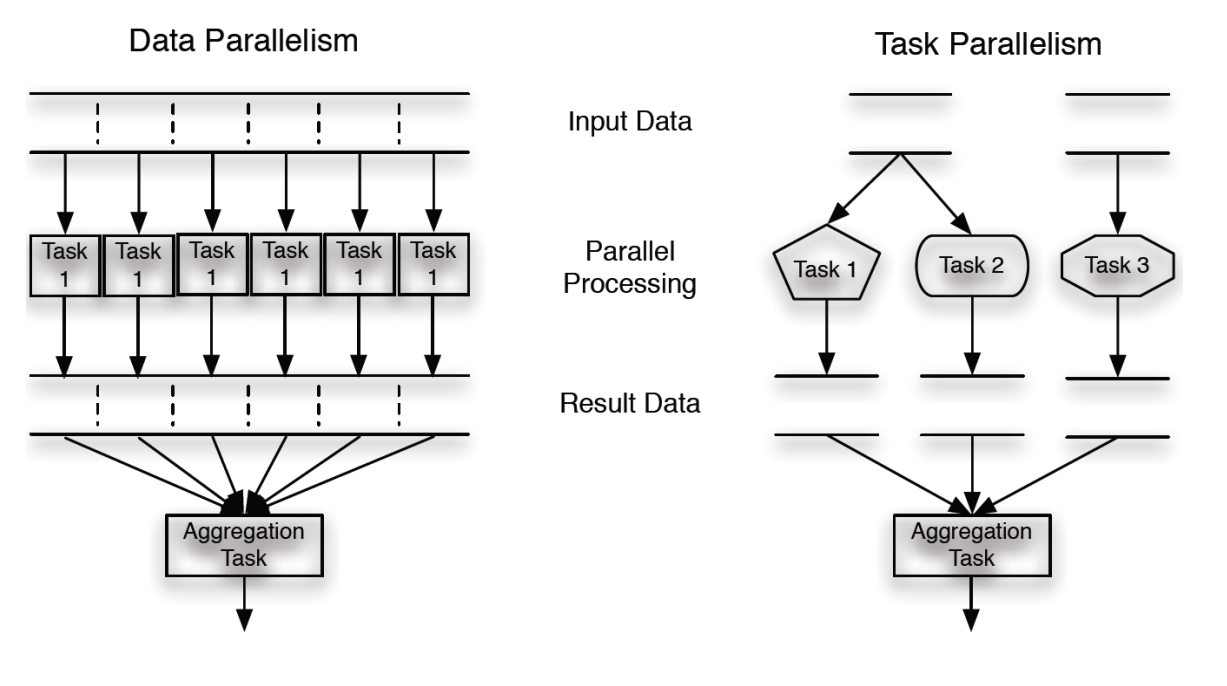
\includegraphics[width=\textwidth]{data-model}
					\caption{Паралелізм задач vs даних}
				\end{figure}
			\end{column}
		\end{columns}
	\end{frame}
	
	\begin{frame}{Архітектура гетерогенних обчислень CUDA}
		\begin{columns}
			\begin{column}{0.5\textwidth}
				\begin{figure}
					\centering
					% Місце для фото: host_device.png
					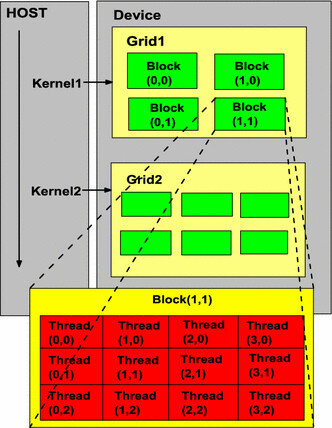
\includegraphics[width=\textwidth]{heterogeneous-model}
					\caption{Модель Host-Device}
				\end{figure}
			\end{column}
			\begin{column}{0.5\textwidth}
				CUDA об'єднує CPU (хост) та GPU (пристрій). Хост керує логікою та пам'яттю, а пристрій виконує масивні обчислення. Оскільки вони мають ізольовані простори пам'яті, програміст повинен явно контролювати копіювання даних через шину PCIe.
			\end{column}
		\end{columns}
	\end{frame}
	
	\begin{frame}{Керування пам'яттю пристрою}
		\begin{block}{Життєвий цикл даних на GPU}
			1. \textbf{cudaMalloc}: Виділення простору у відеопам'яті. \\
			2. \textbf{cudaMemcpy}: Передача даних (HostToDevice). \\
			3. \textbf{Kernel Launch}: Виконання обчислень. \\
			4. \textbf{cudaMemcpy}: Повернення результатів (DeviceToHost). \\
			5. \textbf{cudaFree}: Звільнення ресурсів.
		\end{block}
		\begin{figure}
			\centering
			% Місце для фото: memory_transfer.png
			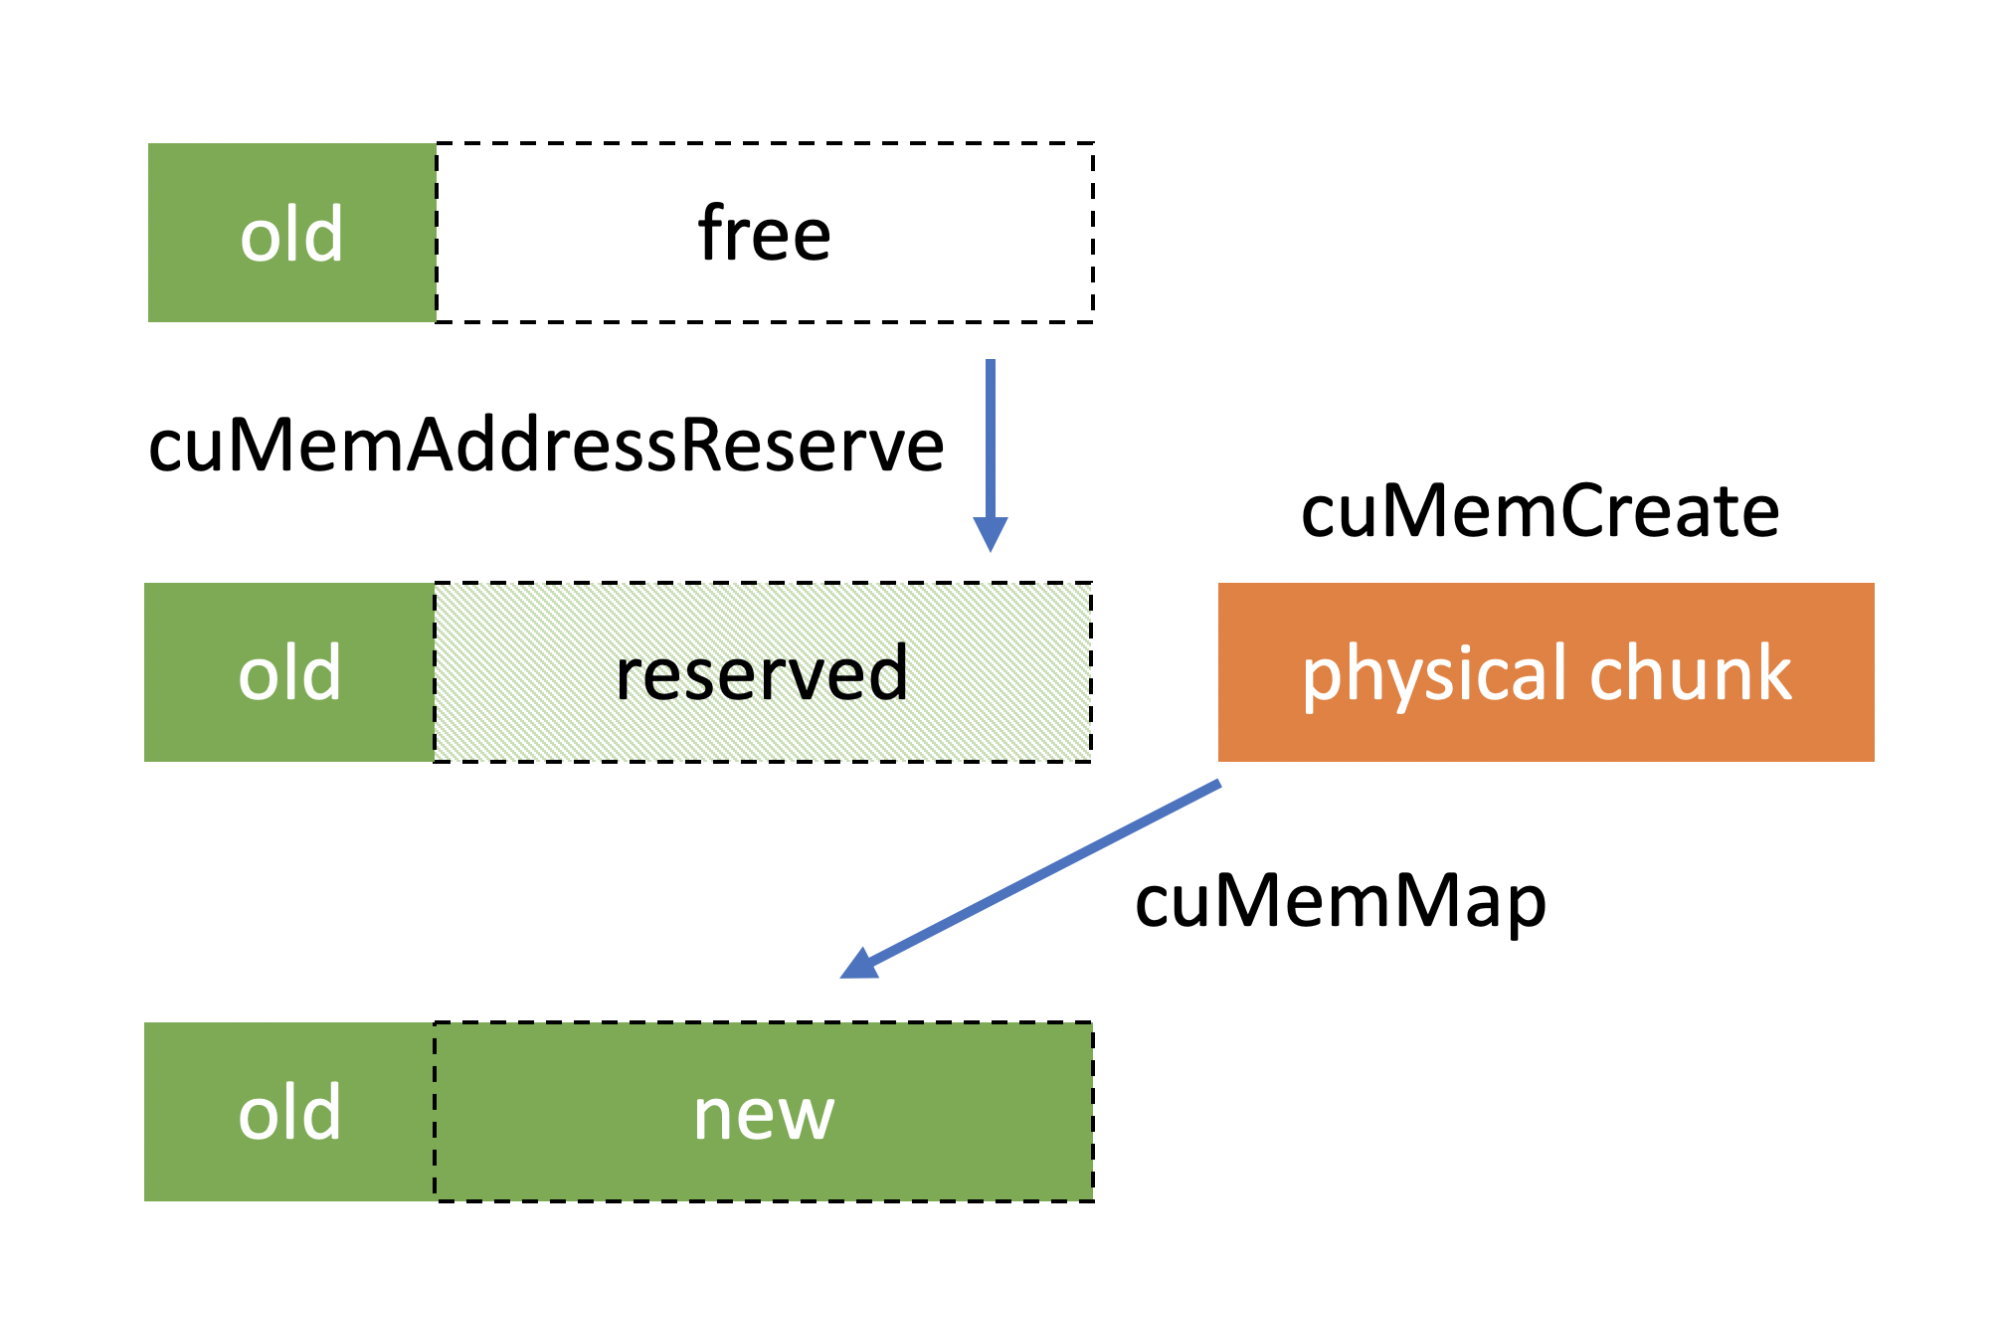
\includegraphics[width=0.5\textwidth]{lifetime}
			\caption{Схема життєвого циклу даних}
		\end{figure}
	\end{frame}
	
	\begin{frame}[fragile]{Написання ядра (Kernel)}
		Код ядра описує логіку для одного потоку. Специфікатор \texttt{\_\_global\_\_} вказує, що функція виконується на GPU.
		\begin{exampleblock}{Vector Addition (CUDA C)}
			\begin{verbatim}
				__global__ 
				void vecAdd(float* A, float* B, float* C, int n) {
					int i = blockDim.x * blockIdx.x + threadIdx.x;
					if (i < n) {
						C[i] = A[i] + B[i];
					}
				}
			\end{verbatim}
		\end{exampleblock}
	\end{frame}
	
	\begin{frame}{Організація потоків (Grids, Blocks, Threads)}
		\begin{columns}
			\begin{column}{0.5\textwidth}
				Потоки об'єднуються в блоки, а блоки -- в сітку (Grid). Така ієрархія дозволяє CUDA працювати на будь-якому GPU, незалежно від кількості фізичних ядер.
				\\ \vspace{0.3cm}
				\textbf{Індексація:} \\
				\texttt{index = blockIdx.x * blockDim.x + threadIdx.x}
			\end{column}
			\begin{column}{0.5\textwidth}
				\begin{figure}
					\centering
					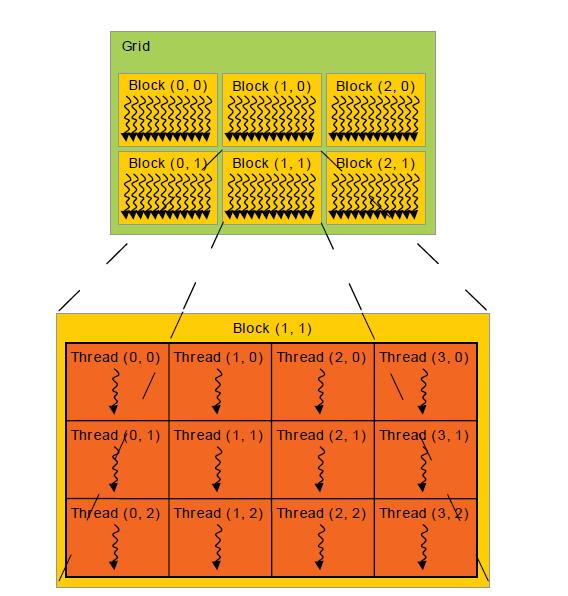
\includegraphics[width=\textwidth]{grid}
					\caption{Ієрархія потоків у CUDA}
				\end{figure}
			\end{column}
		\end{columns}
	\end{frame}
	
	\begin{frame}[fragile]{Rust та безпечні абстракції (Perspectives)}
		Використання Rust дозволяє замінити небезпечні вказівники та ручні індекси безпечними ітераторами.
		\begin{columns}
			\begin{column}{0.5\textwidth}
				\textbf{CUDA C (Низький рівень):}
				\begin{tiny}
					\begin{verbatim}
						// Ризик: out-of-bounds, memory leaks
						cudaMalloc(&d_A, size);
						vecAdd<<<grid, block>>>(d_A, ...);
					\end{verbatim}
				\end{tiny}
			\end{column}
			\begin{column}{0.5\textwidth}
				\textbf{Rust (Високий рівень):}
				\begin{tiny}
					\begin{verbatim}
						// Безпечно: автоматичне керування пам'яттю
						let c: Vec<_> = a.par_iter()
						.zip(&b)
						.map(|(x, y)| x + y)
						.collect();
					\end{verbatim}
				\end{tiny}
			\end{column}
		\end{columns}
		\begin{alertblock}{Переваги Rust-підходу}
			Гарантія безпеки пам'яті (Memory Safety) на етапі компіляції та відсутність станів гонитви (Data Races).
		\end{alertblock}
	\end{frame}
	
	\begin{frame}{Висновки}
		\begin{itemize}
			\item CUDA C -- це фундамент та повний контроль над залізом.
			\item Розуміння ієрархії потоків (SIMT) є критичним для роботи із паралельними даними.
			\item Майбутнє -- за безпечними мовами (Rust) та високорівневими абстракціями (Rayon), що зменшують кількість помилок.
		\end{itemize}
	\end{frame}
	
\end{document}